\section{Archive Process Design}
\subsection{Preconditions Required for an Archive}
Certain preconditions have to be met before an archive process could start to ensure the correctness of the data which are mentioned below:
\begin{enumerate}
    \label{lst:preconditionsArchive}
    \item \textbf{Mark resources:} The MARS framework is a multi user application meaning a project can be accessed by many users at the same time. 
    As multiple users can modify the data simultaneously, it could be possible that someone modifies a resources during an archive. As the 
    Archive service has no way to detect this modification. This would lead inconsistent data being archived.
    Therefore, to avoid this situation the resources must be marked before the start of the archive. The marking would ensure that no other process except the Archive
    service would have access to modify the marked contents during the archive process. The marking process would be handled using the Marking service.
    \item \textbf{Get Metadata for the project:} The metadata contains all necessary information about the files. The scenarios, files and the result 
    configuration depends on these metadata getting 
    the respective data. If the metadata cannot be obtained the archive process cannot continue. 
    \item \textbf{Get Simulation runs:} The simulation runs contains the simulation id which is required to archive the correct simulation id. This dependency
    with simulation run makes it necessary that the simulation runs are obtained before archiving simulation results.
\end{enumerate}

\subsection{Decision for Not Archiving the Project}
The resources depicted in table (Table \ref{table: archivedMars}) must be archived following the MARS resource hierarchy (Figure \ref{fig:marsDependency}).
Following the hierarchy, it is arguable why the project is not being archived, despite it being present. The project lies on the top of the hierarchy 
meaning no other resources are usable without its existence. Section \ref{ssec:retrieveAnalysis} mentions the requirement that the Archive service must 
be able to restore all the resources back into the system. Therefore, during a restore if, a specific project archived
is not available then other resources cannot be brought back into the system as all of them are dependent to the project. To make the restore process possible,
the project data is not archived which now acts as a point of reference to bring back the children resources. 
If the project was to be archived also a mechanism
which ensures that the users referenced in the archive exist in the MARS system (active system). It could happen that during a retrieve the users in an
archived project may not exist anymore as they were removed causing the process to fail. Therefore, this decision also reduces the complexity of the 
archive and restore as this mechanism which is hard to maintain can be avoided.


\subsection{Data Format}
A suitable file format must be chosen because it determines how the data access will be realized and whether it meets
the criteria mentioned in Section \ref{section:functionalReq}. The different types of data archived are the metadatas for files, scenarios, 
result configurations, simulation plans, simulation run including the input files, models and the simulation results. 
The data format that is being discussed in this section mainly focuses on the metadata and they are received originally as a JSON document.
The metadata is very important because they give the system vital information that will be used during retrieve process. 

\subsubsection{HDF5}
HDF5 is a file format for storing and managing data which has support for various data types designed for
efficient I/O which has the capability to support big data \cite{HDF5}. It has been successfully applied to different scientific projects which
involve simulation (Efficient
for simulation data \cite[p.~11]{Savic2007}). This file can also be defined as an abstract data container which includes building blocks for data organization. 
This file system can hold a variety of heterogeneous objects like images, graphs, documents, tables etc. It also has support for a n-dimensional table  \cite[p.~2]{HDF5}. 
The HDF5 format has two primary objects which define the data storage structure:
\begin{enumerate}
    \item \textbf{Groups:}  They are responsible to organize the data objects in the HDF5 file format. A group can be compared to a directory 
    in Windows or a Unix system \cite{HDF5}. Figure \ref{fig:HDF5} shows an example of a Group in a HDF5 file. Using the API of the HDF5 libraries a Dataset 
    (e.g. Dataset1) can be accessed via the path name (e.g. /Root/Group1/Dataset1).
    \item \textbf{Datasets:} A dataset can be defined as a multidimensional array of data. This object contains the raw/actual data which one would like to store (e.g. simulation results).
    These data are stored in a tabular format 
    one can specify the different data types for the raw data i.e. integer, float, character, variable length strings \cite{HDF5}. Figure \ref{fig:dataset} shows
    an example of a Dataset in a HDF5 file which is stored in a an array.
\end{enumerate}
%The Groups in the 

\begin{figure}[H]
    \centering 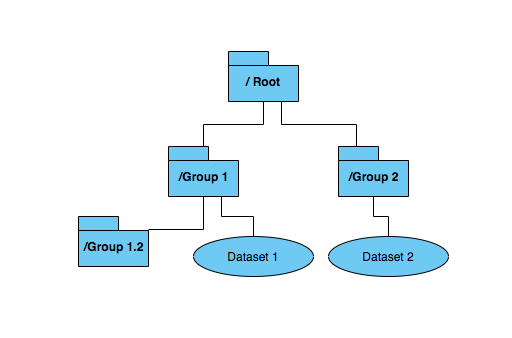
\includegraphics[scale=0.6]{grafiken/groupsHDF5.png}
    \caption{HDF5 Groups \cite{HDF5}}
    \label{fig:HDF5}
\end{figure}

\begin{figure}[H]
    \centering 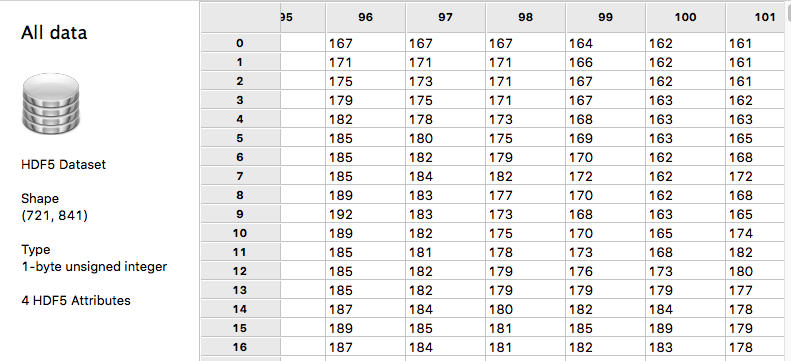
\includegraphics[scale=0.45]{grafiken/dataset.png}
    \caption{Example of a HDF5 dataset}
    \label{fig:dataset}
\end{figure}

\subsubsection{JSON} 
JSON(JavaScript Object Notation) is a data format which is very easy for humans and machines to read and write. This format is
completely language independent which follows the conventions used in different programming languages i.e. C\#, Java, Python and more. The REST API implemented in the
MARS framework support this format with ease making this a very suitable candidate. This format is widely 
accepted and even MongoDB supports it without any problem. Also, MongoDB seems to be a good candidate but the requirement (Section \ref{sec:anaCompress}) states that the archived
data should be easily accessible to a non expert and using MongoDB requires some amount of technical expertise.


\subsubsection{Conclusion}
   After careful consideration,  
    it seems so that HDF5 file formats is not suitable for the archive and retrieve process.      
    To store the data in an HDF5 format the JSON formated metadata must be parsed first and then
    be stored in the multidimensional array structure of HDF5. Since it is very complicated to parse the metadata of different models this
    file format will not be used for this thesis. 

    Lastly, the file format for archive is planned to be JSON for the metadata files i.e. simulation runs, simulation plans, scenarios and, result configuration. All the project resources will be packed inside a folder in the Synology (See Figure \ref{fig:synology})
    which is easily accessible via the MARS network. The decision to use JSON is due to the fact that the API in the MARS back end services 
    use the JSON structure to communicate. Using this structure simplifies the process of archive and also retrieve as the metadata can be easily saved.
\begin{figure}[H]
    \centering 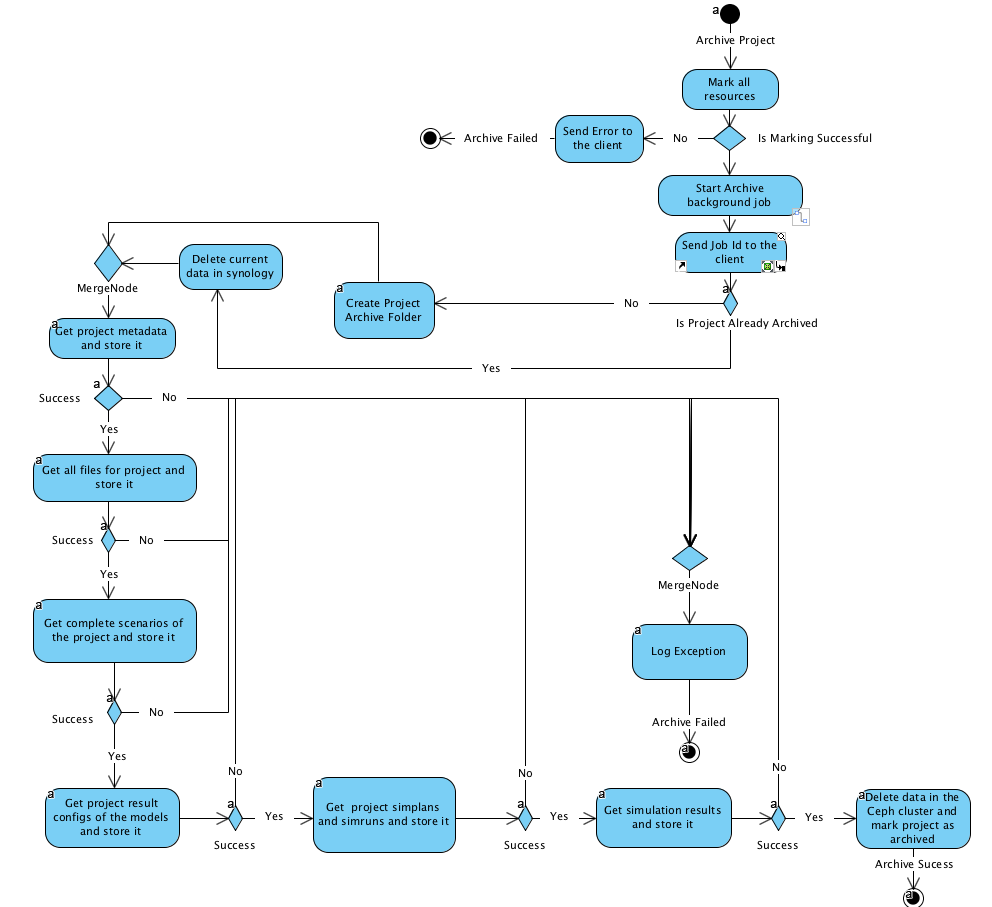
\includegraphics[scale=0.45]{grafiken/archiveActivity.png}
    \caption{Activity Diagram of MARS project Archive process}
    \label{fig:archiveActivity}
\end{figure}

Figure \ref{fig:archiveActivity} illustrates an activity diagram of archiving an entire archive process. As mentioned in Section \ref{lst:preconditionsArchive},
marking the resources for the project is the first requirement needed to start the process. If the project resources are marked successfully
then the archive would be initialized as a background job and the job id would be send to the client. In case the marking would fail the error message will be 
sent to the client and the archive process will halt. The archiving process is visioned to be a background job due to the fact that a single process could take
a long period of time and would block the server for additional requests. Following the successful job creation, the process checks if an archive already
exists. A check for an existing project is made to ensure that if the archive process failed is caused by an transient error, the incomplete data can be removed. After
the archive folder creation, the metadata, files, scenarios, result configurations, simulation plans, simulation runs and the simulation results are retrieved respectively.
After a successful archive process the  resources are deleted from the Ceph cluster. Lastly, in case of some failures during archiving the exception will be logged 
which can be later analyzed for maintenance.

\begin{figure}[H]
    \centering 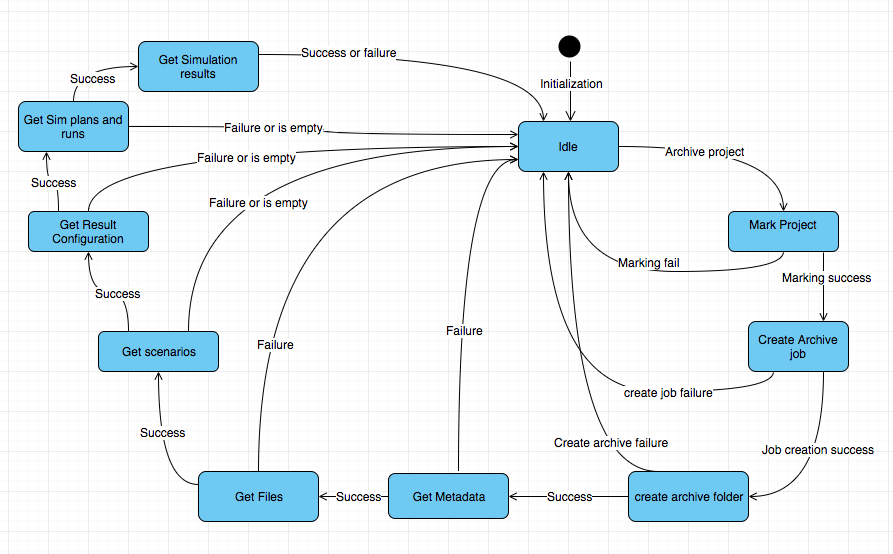
\includegraphics[scale=0.45]{grafiken/stateArchive.png}
    \caption{State Diagram of MARS project Archive process considering empty states}
    \label{fig:stateArchive}
\end{figure}

Figure \ref{fig:stateArchive} illustrates the transitions that can occur during the archive process. The idle state refers to the state where no archive process
is being executed. Additionally, the state digram also considers
how the state would change if one of the resources are empty. In the case of an empty resource (e.g. no scenarios available for the project) the archive
process stops gracefully and transitions to the idle state. 

\begin{figure}[H]
    \centering 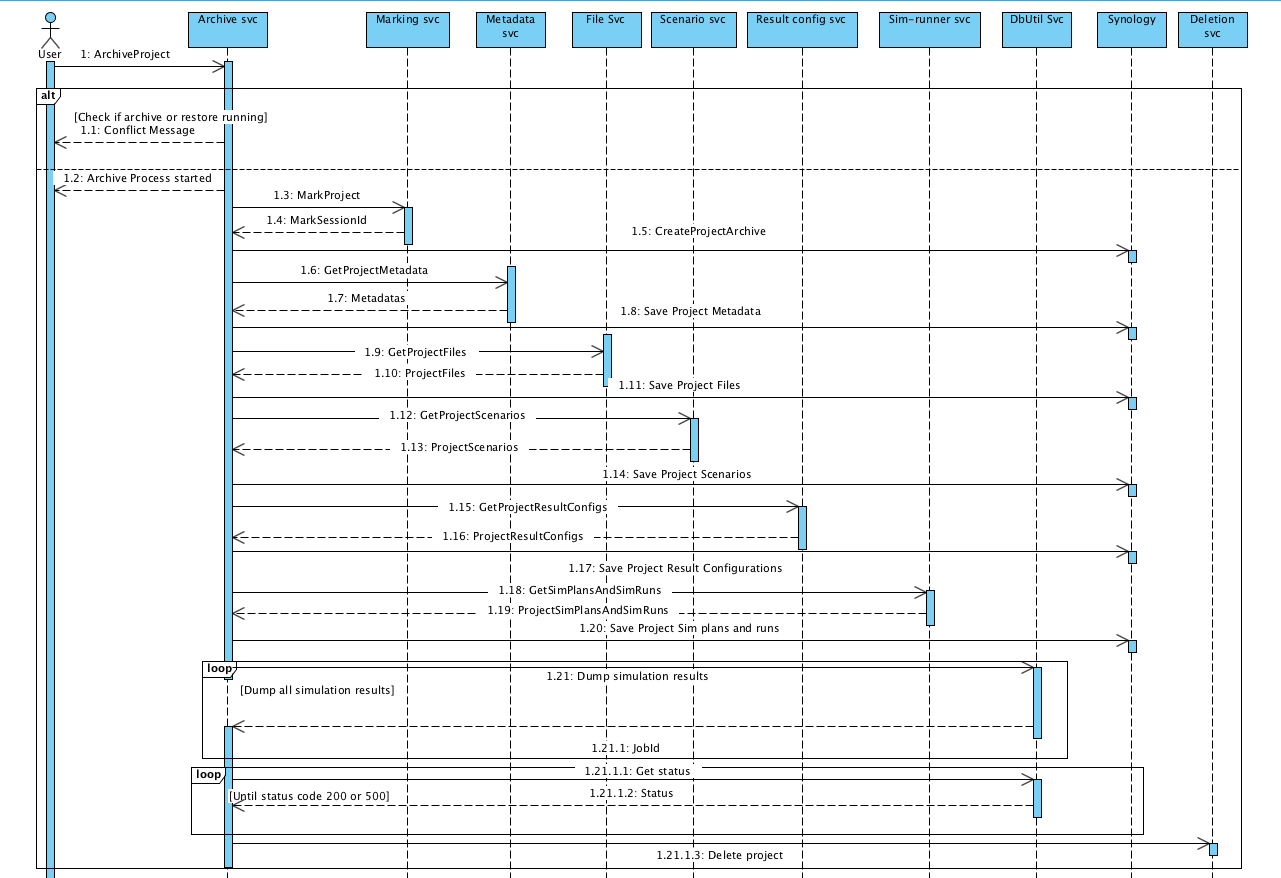
\includegraphics[scale=0.5, angle=90, origin=c]{grafiken/sequenceArchive.png}
    \caption{Sequence Diagram for the Archive process}
    \label{fig:sequenceArchive}
\end{figure}

Figure \ref{fig:sequenceArchive} illustrates the Sequence diagram for a complete archive process. The first step after an archive request would be to check
whether an archive or retrieve process for the current project is under progress. In case the process is in progress the archive request would be denied to the
user with an conflict message. If no process with the project is running then an archive job (a separate thread) would be created and a message to the client with start of archive process would be
sent. Following the job creation the project will be marked so that during archive no changes to the project resources could be made. If this step fails the archive 
process would stop by logging the error. After marking step completes the archive process receives a mark session id and the dependent resources which would allow the process to make
changes to the resources. Using the dependent resources the process retrieves metadata, files, scenarios, result configurations, simulation plans, simulation runs 
respectively and persists them in Synology. Lastly, the simulation result dump action will be called which will archive the result data. The process waits until
all the result data is archived successfully. After a successful archive a request to delete the project data would be made so that the system memory can be freed.

A major issue to be discussed is when the archive process fails which requires a rollback by unmarking the project. As mentioned earlier the project is
marked as "TO\_BE\_ARCHIVED" so that no other processes can modify the contents during the archive process. This is a great strategy if everything goes as planned but 
often enough this is not the case and it is mandatory that an unmarking of the project is done otherwise the project would be unusable. It also happens that since the
marking service is dependent upon many services it has a very high rate of failure as well. This brings upon the problem how would the archive service behave if the
unmarking of the project fails. It seems very natural to just repeat the process until the unmarking request would succeed since it is absolutely necessary to unmark
a project. If this happens only with a single process it does not make a huge difference but thinking of the bigger picture if this 
occurs with 100 different processes at the same time, it would use valuable processing resources as it may be stuck in a deadlock condition until a outside interruption
is made. To avoid this a fixed number of retries to unmark the project with certain time interval for the request 
will be made. Although, this solves the issue of using up resources but the problem that the project is unusable is still there. No other way except a manual unmarking is seen so 
it is decided that the archive process would also persist the marking session id which can be used to call the unmarking endpoint. With the use of this id a manual 
trigger is possible as soon as the error is fixed. The marking session id can be easily retrieved also from the GUI as it will be included in the status request of
the archive job.
 